\section{Case study: slick-direct} % (fold)
\label{sec:CaseStudy}
Slick is a popular Scala library.
Slick is recommended by Typesafe as the functional relational mapper for their well known Play framework.
Professional Scala consultancies such as \href{http://underscore.io}{underscore.io} offer public and private training on Slick and underscore.io even recently released a book about the library\footnote{http://underscore.io/training/courses/essential-slick/}.
The hefty prices on the private training indicates that there is commercial interest in using Slick.
The fact that the book is close to 300 pages may also indicate that the library has a steep learning curve.

We chose to evaluate Directembedding by implementing a front-end for Slick for a few reasons.
Firstly, Slick is a widely used library in the industry.
Secondly, the lifted embedding API is quite elaborate and uses many advanced features of the Scala type system.
Thirdly, there exists a lot of related work on direct embedding for Slick.

In this case study, we compare in detail the lifted embedding with our implementation of the direct embedding.
Sections~\ref{sub:LiftedEmbedding} and~\ref{sub:LiftedEmbedding} cover how queries are created in the lifted embedding and direct embedding, respectively.
In Section~\ref{sub:TypeSignatures}, we look into the differences between the type signatures in the lifted embedding and direct embedding.
In particular, we consider the trade-offs that we took to implement slick-direct.
In Section~\ref{sub:Relatedwork}, we look at the related work on direct embedding with Slick.

\subsection{Lifted embedding} % (fold)
\label{sub:LiftedEmbedding}
The lifted embedding is the recommended way to query data with Slick.
The supertype of all members in the lifted embedding is the \texttt{slick.lifted.Rep[T]} trait.
Figure~\ref{fig:rep} shows the type hierarchy of \texttt{Rep[T]}.
To create a query with the lifted embedding, a Slick user must in one way or another interact with all subtypes in the hierarchy.
\begin{figure}
    \centering
    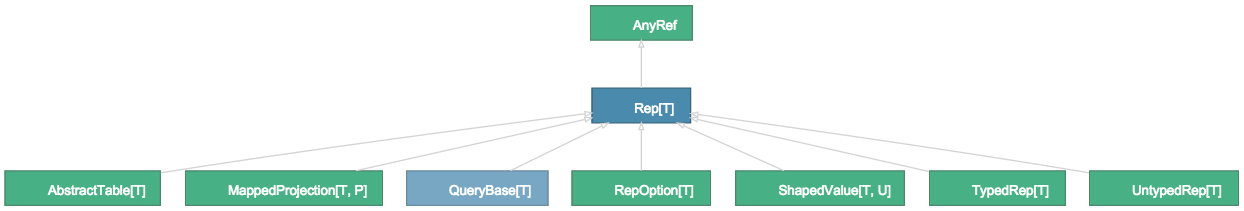
\includegraphics[width=\textwidth]{img/rep.png}
    \caption{The type hierarchy of \texttt{slick.lifted.Rep[T]} in Slick.}\label{fig:rep}
\end{figure}
The purpose of the lifted embedding API is to create an abstract syntax tree (AST) of type \texttt{slick.ast.Node}, which is then passed onto the query optimization engine of Slick.
In the next few paragraphs, we will follow an example to see how a query inside the lifted embedding is created from the point of view of a Slick users.
The \texttt{Node} API will not be discussed until Section~\ref{sub:alternatives}.
The following example is made up of simple database of users and cars owned our users and is split into four steps.
Observe that some details such as database drivers are left out for clarity.
% Figure~\ref{fig:node} shows the type hierarchy of \texttt{Node}.
% \begin{figure}
%     \centering
%     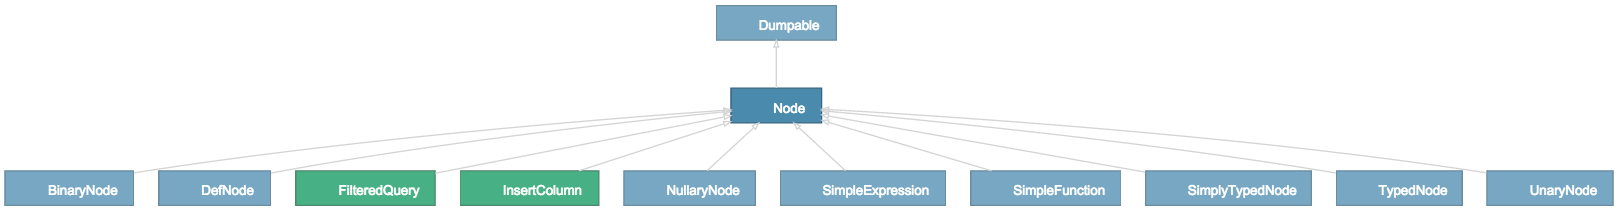
\includegraphics[width=\textwidth]{img/node.png}
%     \caption{The type hierarchy of \texttt{slick.ast.Node} in Slick.}\label{fig:node}
% \end{figure}


First, we define our Scala case classes for our \texttt{User} and \texttt{Car} objects.
\lstinputlisting{code/oo.scala}
These classes will be the values which we want to insert into and fetch from our database.

Second, to provide necessary metadata to query on our user and car objects, we define a \texttt{Table}.
\lstinputlisting{code/table.scala}
Observe that the names of the members in our standard user and car objects are repeated at least four times: 
\begin{inparaenum}[i)]
    \item in the case class definition,
    \item in the method names in the table definition,
    \item in the string literals to identify the column names in the database, and
    \item in the \texttt{ProvenShape} mapping in the \texttt{$\ast$} method.
\end{inparaenum}
In the case of the \texttt{ownerId} --- which has the foreign key constraint --- we must repeat the name two more times, a combined of six times.
The benefit to this table definition is that it gives great flexibility to the user.
The downside is that the table definition forces a lot of boilerplate onto users --- violates DRY --- and may be likely to introduce bugs in the code.
To alleviate this issue, Slick provides a library to generate these table definitions from a database schema.

Third, to write queries we create \texttt{TableQuery} objects.
\lstinputlisting{code/tablequery.scala}
Queries are written with a similar syntax as Scala collections are operated.
\lstinputlisting{code/example-queries.scala}
Once we invoke a \texttt{map} or \texttt{filter} operation on a \texttt{TableQuery[T]}, we get a value of type \texttt{Query[E, T, C]} where in our example
\begin{inparaenum}[i)]
\item \texttt{E} will be \texttt{Users} and \texttt{Cars}, 
\item \texttt{T} will be \texttt{User} and \texttt{Car}, and
\item \texttt{C} will typically be the collections container \texttt{Seq[T]}.
\end{inparaenum}

Fourth, we run our queries on a database object.
In Slick 3.0, the argument supplied to the database object is of type \texttt{DBIOAction[T]}, and the database returns a values of type \texttt{T}, which will be in our case Users.

\subsection{Direct embedding} % (fold)
\label{sub:Directembedding}

\begin{itemize}
    \item Missing features.
\end{itemize}

% subsection Direct embedding (end)

\subsection{Comparing type signatures} % (fold)
\label{sub:TypeSignatures}
% subsection Querying (end)
Slick-direct currently supports 6 categories of queries.
Each of these categories has a test suite showing comparison of the slick-direct API and the lifted embedding in the Slick library.
Herein, we highlight three major differences between the two querying APIs.
In all examples, assume the type of \texttt{this} to be \texttt{lifted.Query[E, T, \_]} for \texttt{direct.Query[T, \_]}, respectively.
\lstinputlisting[caption=Map API]{code/map.scala}
In order to guarantee that \texttt{f} produces a value that can be persisted into a database, \texttt{lifted.Query} adds an implicit shape parameter on the type of \texttt{F}.
Slick-direct eliminates the need for this shape parameter by not supporting selection of more than one column.

\lstinputlisting[caption=Filter API]{code/filter.scala}
In order to guarantee that \texttt{f} produces a value that can be a boolean condition, \texttt{lifted.Query} adds an implicit \texttt{CanBeQueryCondition} parameter on the type of \texttt{T}.
Slick-direct eliminates the need for this implicit parameter by forcing the method to be of type \texttt{T => Boolean}.
The issue with this elimination is that query conditions on wrapped column types such as \texttt{Option[Boolean]}cannot be supported.

\lstinputlisting[caption=Join API]{code/join.scala}
This example may be a bit unfair against \texttt{lifted.Query}, but shows that type signatures in the lifted embedding can become unwieldy complicated.
The type signature of the equivalent method in slick-direct is undeniably more user-friendly.

For more examples of queries supported by slick-direct, please refers to the test suites provided in the project's repository, linked at the end of this report.


% subsection Working with Slick (end)
\subsection{Alternative approaches} % (fold)
\label{sub:alternatives}

\subsection{Related work} % (fold)
\label{sub:Relatedwork}
There have been made two attempts to provide a simplified Query API to Slick using macros.

\begin{sloppypar}
The first attempt was made by the Slick team and resulted in a direct embedding API which has now been deprecated and will be removed in the upcoming 3.1 release of Slick.
The approach taken with the direct embedding API differs greatly from our approach in slick-direct.
The Queryable API from the direct embedding implemented a separate macro for each method and produced values of type \texttt{ast.Node}, obviating the need for the \texttt{lifted.Query}.
Slick-direct, on the other hand, implements one macro logic for all invocations on our Query API and produces values of type \texttt{lifted.Query}.
Slick-direct does not implement any query logic, it delegates it to \texttt{lifted.Query}.
\end{sloppypar}

The second attempt was a made by Amir Shaikhha~\autocite{shaikhha_embedded_2014} using the Yin-Yang Framework~\autocite{jovanovic_yin-yang:_2014}.
The approach taken in this second attempt is similar to the approach taken in our case in many ways.
The library implements one macro to reify values in a shallow Query API.\
However, this second attempt produced values in a shadow embedding that operates on values of type \texttt{lifted.Query} at runtime.
The main difference between our case study and this attempt is that Directembedding obviates the need for the shadow embedding by transforming in one step the values in the shallow embedding into the deep embedding.

Due to time constraint, we implemented only a subset of the methods supported in the previous two attempts.
Nevertheless, we consider that we picked the methods that introduced the most interesting challenges for our purposes.
We believe that the remaining methods that are not supported in our case study could be added to our API with a small additional effort.



% section Evaluation: slick-direct (end)

% TODO: Custom column types, which are supported in slick-direct
% TODO: Just.... MORE!!!!!!!!!!!!!!

